\documentclass[border=6pt]{standalone}
\usepackage[T1]{fontenc}
\usepackage[utf8]{inputenc}
\usepackage[scaled=0.98]{helvet}
\renewcommand{\familydefault}{\sfdefault}
\usepackage{amsmath}
\usepackage{graphicx}
\graphicspath{{../../../../../../exercises_lecturenotes/lecture_notes/kurs100_lektionsnoter/}}
\usepackage{tikz}
\usepackage{pgfplots}
\pgfplotsset{compat=1.18}
\usetikzlibrary{arrows.meta, decorations.pathreplacing, calc, positioning, fit, backgrounds, shapes.geometric}
\usepgfplotslibrary{groupplots,fillbetween}
\definecolor{scanpink}{HTML}{E5006D}
\definecolor{scanteal}{HTML}{00A6A6}
\definecolor{scannavy}{HTML}{243746}
\definecolor{scanlightgray}{HTML}{F1F2F3}
\begin{document}
  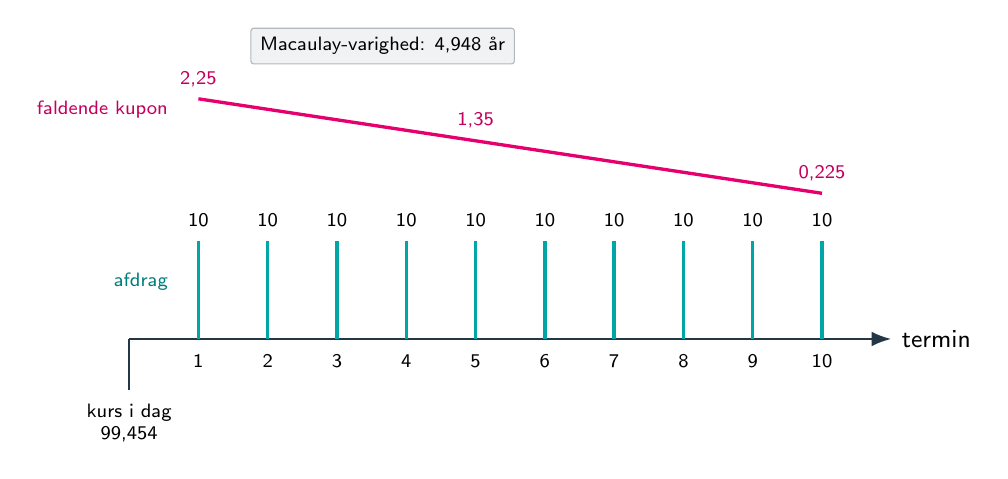
\begin{tikzpicture}[
      x=0.88cm,
      y=1cm,
      font=\small,
      timeline/.style={
        -{Latex[length=2.5mm]},
        line width=0.9pt,
        draw=scannavy
      },
      payment/.style={
        line width=1.2pt,
        draw=scanteal
      }
  ]

    \draw[timeline] (0,0) -- (11,0) node[right] {termin};

    \foreach \x in {1,...,10} {
      \draw[payment] (\x,0) -- (\x,1.25);
      \node[font=\scriptsize, anchor=south] at (\x,1.30) {10};
      \node[font=\scriptsize, anchor=north] at (\x,-0.08) {\x};
    }

    \node[
      font=\scriptsize,
      anchor=e,
      scanteal!75!black
    ] at (0.7,0.75) {afdrag};

    % Faldende kuponbetaling
    \draw[scanpink, very thick]
      (1,3.05) -- (10,1.85);

    \node[
      font=\scriptsize,
      anchor=south,
      scanpink!85!black
    ] at (1,3.08) {2,25};

    \node[
      font=\scriptsize,
      anchor=south,
      scanpink!85!black
    ] at (5,2.55) {1,35};

    \node[
      font=\scriptsize,
      anchor=south,
      scanpink!85!black
    ] at (10,1.88) {0,225};

    \node[
      font=\scriptsize,
      anchor=e,
      scanpink!85!black
    ] at (0.7,2.95) {faldende kupon};

    % Kurs i dag
    \draw[scannavy, line width=0.8pt]
      (0,0) -- (0,-0.65);

    \node[
      font=\scriptsize,
      anchor=north,
      align=center
    ] at (0,-0.7) {
      kurs i dag\\
      99,454
    };

    % Macaulay-varighed
    \node[
      draw=scannavy!35,
      fill=scanlightgray,
      rounded corners=1pt,
      font=\scriptsize,
      anchor=west
    ] at (1.75,3.72) {
      Macaulay-varighed: 4,948 år
    };

  \end{tikzpicture}
\end{document}
